\textbf{Pour cette première partie, aucune justification n'est demandée et une seule réponse est possible par question. Pour chaque question, reportez son numéro sur votre copie et indiquez votre réponse.}

	Une réponse fausse ou l'absence de réponse n'enlève aucun point.

	\textbf{Question 1}

	Le nombre \quad $\dfrac{1}{2}+\dfrac{3}{2} \times 4$ \quad est égal à :

	\begin{tblr}{XXXX}
			\textbf{A.} 8 & \textbf{B.} $\dfrac{13}{2}$ & \textbf{C.} 4 & \textbf{D.} $\dfrac{16}{8}$ \\
		\end{tblr}

	\medskip

	\textbf{Question 2}

	Le volume de la partie visible d'un iceberg est d'environ 10~\% de son volume total.

	Si la partie visible d'un iceberg est de $\np[km^3]{150}$, quel sera le volume total de cet iceberg ?

	\begin{tblr}{XXXX}
		\textbf{A.} $\np[km^3]{1350}$ & \textbf{B.} $\np[km^3]{1500}$ & \textbf{C.} $\np[km^3]{15}$ & \textbf{D.} $\np[km^3]{135}$ \\
	\end{tblr}

	\medskip

	\textbf{Question 3}

	Le prix d'un article est multiplié par 0,845. Cela signifie que le prix de cet article a :

	\begin{tblr}{XX}
		\textbf{A.} augmenté de 84,5~\% & \textbf{B.} baissé de 1,55~\% \\
		\textbf{C.} augmenté de 15,5~\% & \textbf{D.} baissé de 15,5~\% \\
	\end{tblr}

	\medskip

	\textbf{Question 4}

	On considère la fonction A définie pour tout réel $x$ par :
	\[A(x)=(x+5)(x+8)\]
	Le tableau de signes de $A(x)$ sur $\R$ est :

	\begin{tblr}{XX}
		\textbf{A.} \begin{tikzpicture}[baseline={(F0.base)}]
			\tkzTabInit[lgt=1,espcl=1.4]{$x$/0.7, $A(x)$/0.7}
			{$-\infty$,$-8$,$-5$,$+\infty$}
			\tkzTabLine{,-,z,+,z,-}
		\end{tikzpicture}&
		\textbf{B.} \begin{tikzpicture}[baseline={(F0.base)}]
			\tkzTabInit[lgt=1,espcl=2.1]{$x$/0.7, $A(x)$/0.7}
			{$-\infty$,$-5$,$+\infty$}
			\tkzTabLine{,-,z,+}
		\end{tikzpicture}\\
		\textbf{C.} \begin{tikzpicture}[baseline={(F0.base)}]
			\tkzTabInit[lgt=1,espcl=1.4]{$x$/0.7, $A(x)$/0.7}
			{$-\infty$,$-8$,$-5$,$+\infty$}
			\tkzTabLine{,+,z,-,z,+,}
		\end{tikzpicture}&
		\textbf{D.} \begin{tikzpicture}[baseline={(F0.base)}]
			\tkzTabInit[lgt=1,espcl=1.4]{$x$/0.7, $A(x)$/0.7}
			{$-\infty$,$5$,$8$,$+\infty$}
			\tkzTabLine{,+,z,-,z,+,}
		\end{tikzpicture}\\
	\end{tblr}

	\medskip

	\textbf{Question 5}

	Un singe choisit une lettre au hasard parmi les lettres de l'alphabet.

	On note les évènements :

	\begin{itemize}[left=5mm,label={\textbullet~~}]
		\item $V$ : \og Le singe choisit une voyelle. \fg{}
		\item $M$ : \og Le singe choisit une des lettres du mot SINGE. \fg{}
	\end{itemize}

	\emph{Rappel :} L'alphabet est constitué de 26 lettres dont les voyelles sont : A, E, I, O, U, Y.

	On note $P_{M}(V)$ la probabilité que le singe choisisse une voyelle sachant qu'il a choisi une lettre du mot SINGE. On peut alors affirmer que $P_{M}(V)$ vaut :

	\begin{tblr}{XXXX}
		\textbf{A.} $\dfrac{6}{26}$&
		\textbf{B.} $\dfrac{2}{5}$&
		\textbf{C.} $\dfrac{2}{6}$&
		\textbf{D.} $\dfrac{5}{6}$
	\end{tblr}

	\medskip

	\begin{minipage}{0.5\linewidth}
	\textbf{Question 6}

	Soit $f$ une fonction affine, dont on a tracé la représentation graphique dans le repère ci-contre.\\

	Une expression algébrique de $f$ est :\\

	\begin{tblr}{XX}
		\textbf{A.} $f(x) = -x + 30$ &
		\textbf{B.} $f(x) = 30 x + 3$ \\
		\textbf{C.} $f(x) = -10 x + 30$ &
		\textbf{D.} $f(x) = -\dfrac{1}{10} x + 30$ \\
	\end{tblr}
	\end{minipage}
	\hfill
	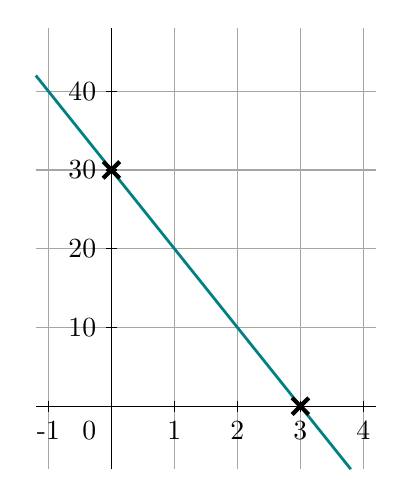
\begin{tikzpicture}[x = 8mm, y = 1mm, baseline={(current bounding box.center)}]
		\draw[gray!70, xstep=1,ystep=10] (-1.2,-8) grid (4.2,48);
		\draw (-1.2,0)--(4.2,0)
			(0,-8)--(0,48);
		\foreach \x in {-1,1,2,3,4}{
			\draw (\x,2pt)--(\x,-2pt) node[below]{\x};}
		\foreach \y in {10,20,30,40}{
			\draw (2pt,\y)--(-2pt,\y) node[left]{\y};}
		\node[below left] (O) at(-2pt,-2pt) {0};
		\draw[teal,line width=1pt] (-1.2,42)--(3.8,-8) ;
		\foreach \c in {{(3,0)},{(0,30)}}{
			\draw[line width=1.5pt,shift={\c}] (3pt,3pt)--(-3pt,-3pt) (3pt,-3pt)--(-3pt,3pt);}
	\end{tikzpicture}\hfill~











	\medskip

	\textbf{Question 7}

	La forme développée et réduite de l'expression \quad $(x+2)^{2}-(1-x)^{2}$ \quad vaut :

	\begin{tblr}{XXXX}
		\textbf{A.} $2 x^{2}+3$ &
		\textbf{B.} $6 x+3$ &
		\textbf{C.} $2 x+5$ &
		\textbf{D.} $2 x^{2}+2 x+3$ \\
	\end{tblr}

	\medskip

	\textbf{Question 8}

	L'équation \quad $2(x-4)-(2 x+1)=0$\quad admet :

	\begin{tblr}{XX}
		\textbf{A.} Deux solutions : 4 et $\dfrac{1}{2}$ &
		\textbf{B.} Deux solutions : 4 et $-\dfrac{1}{2}$ \\
		\textbf{C.} Aucune solution &
		\textbf{D.} Une infinité de solutions \\
	\end{tblr}

	\medskip

	\textbf{Question 9}

	On considère le nombre réel : \quad $\text{E} =\dfrac{2 \times 3^{2}}{27 \times 2^{3}}$. \quad On peut affirmer que E est égal à :

	\begin{tblr}{XXXX}
		\textbf{A.} $\dfrac{1}{9}$&
		\textbf{B.} $\dfrac{1}{12}$&
		\textbf{C.} 12&
		\textbf{D.} $\dfrac{1}{6}$
	\end{tblr}
